%!TEX TS-program = xelatex
%!TEX encoding = UTF-8 Unicode

\documentclass[12pt]{report}
\usepackage[a4paper]{geometry} 
\usepackage{graphicx}
\usepackage{amssymb,amsmath,amsthm}		% AMS 標準套件
\usepackage{booktabs}						% 表格線條
\usepackage{hyperref}							% 使用 \url 等指令
\usepackage{titlesec} 							% 美化章節標題套件
\usepackage{minted}							% 程式碼
\usepackage{tikz}								% 使用 tikz 套件

\graphicspath{{images/}} 						% 設定圖形路徑


% === 中文 xeCJK 設定 ===
\usepackage{xeCJK}
\setCJKmainfont[BoldFont={cwTeX Q Hei Bold}]{cwTeX Q Ming Medium} % 設預設中文字型及預設粗體
\setCJKfamilyfont{kai}{cwTeX Q Kai Medium}			    				% 楷書	      			
\setCJKfamilyfont{hei}{cwTeX Q Hei Bold}							% 黑體
\setCJKfamilyfont{ming}{cwTeX Q Ming Medium}						% 明體
\setCJKfamilyfont{yuan}{cwTeX Q Yuan Medium}						% 圓體
\setCJKfamilyfont{fsong}{cwTeX Q Fangsong Medium}					% 仿宋體

\newcommand{\kai}[1]{{\CJKfamily{kai}#1}}   			% 用 \kai{使用楷書}
\newcommand{\hei}[1]{{\CJKfamily{hei}#1}}   			% 用 \hei{使用黑體}
\newcommand{\ming}[1]{{\CJKfamily{ming}#1}}		% 用 \ming{使用明體}
\newcommand{\yuan}[1]{{\CJKfamily{yuan}#1}}		% 用 \yuan{使用圓體}
\newcommand{\fsong}[1]{{\CJKfamily{fsong}#1}}		% 用 \fsong{使用仿宋體}

\setromanfont[Mapping=tex-text]{Times} 						% 指定英文字型, 並用 LaTeX 引號
\setsansfont[Scale=MatchLowercase,Mapping=tex-text]{Arial}		% 指定無描邊字型
\setmonofont[Scale=MatchLowercase]{Courier} 					% 指定等寛字型



% === 排版設定 ===
\setlength{\parindent}{0pt}  	% 設定縮排
\linespread{1.2} 				% 設定行距
\setlength{\parskip}{15pt} 		% 設定段落間距


% === 自訂指令 ===
\newcommand{\cmd}{\texttt}
\renewcommand\contentsname{目~錄~}
\renewcommand\listfigurename{圖~目~錄}
\renewcommand\listtablename{表~目~錄}


% === 章節標題 (配合 titlesec) ===
\titleformat{\chapter}[display]
	{\bf\Large}
	{\filleft 第 \thechapter\ 章}
	{1ex}
	{\Huge\titlerule
	 \vspace{2ex}%
	 \filright}
	[\vspace{2ex}%
	 \titlerule]

\title{\hei{中英文 \LaTeX{} 安裝與應用}}
\author{蔡炎龍\\政治大學應用數學系}
\date{2014 年 ver1.0}

\begin{document}
\maketitle


\tableofcontents
\chapter{前言}
開始要學習 \LaTeX, 第一件事情就是安裝。以前安裝 \LaTeX{} 是一件複雜的工作, 尤其是要支中文的 \LaTeX{} 系統。我還記得多年前第一次在 Mac 上安裝 CJK-\LaTeX, 是在 \cmd{oikos.com} 上面有熱心的網友指導, 花了好幾天, 中文字型還需要自己轉, 最後終於完成。完成以後其實我也沒有把握再做一次, 所以之後不管是自己換電腦, 或是朋友要安裝, 我都是把裝好的、包括實驗過程中的垃圾檔案, 一一拷貝過去。

現在, 在很多熱心人士的努力之下, 不管在什麼樣的系統下安裝中文 \LaTeX{} 都不再是難事, 其實不論在 Mac OS, Linux, Windows 上主流的 \TeX{} 系統, 中文套件和基本字型都有了! 如果像本文使用 Xe\LaTeX, 你甚至可以用自己電腦的字型, 不用另外安裝 \TeX{} 專用字型。

使用 \LaTeX, 我們需要良好的編輯程式。事實上任何的文字編輯器都可以, 不過在沒有其他個人偏好的情況下, 我們推薦:

\begin{itemize}
\item TeXWorks (Windows, Linux)
\item TeXShop (Mac OS X)
\end{itemize}

在 Mac OS 和 Windows 的 TeX{} 系統其實都會幫你裝好這些東西。

最後, \LaTeX{} 有個很好的文獻管理搭檔, 叫 Bib\TeX{}。支援 Bib\TeX{} 的文件管理程式一方面可以產生 \LaTeX{} 需要的文獻, 一方面又可以協助我們平時的論文管理。我們這裡推薦使用的程式是:
\begin{itemize}
\item JabRef (Windows, Linux)
\item BibDesk (Mac OS X)
\end{itemize}

我們選擇的程式, 必需是:
\begin{itemize}
\item 簡潔好用 (我不喜歡肥大的程式)
\item 免費 (最好是自由軟體)
\end{itemize}

所以, 在各平台上使用中文 \LaTeX, 不用花錢就可以辦到! 我們以下以 Windows, Mac OS X, 及 Linux 三個平台, 介紹如何安裝 \LaTeX{} 的環境。

%%%
\chapter{Windwos 下的 \LaTeX}
在 Windows 下我們需要安裝以下程式、字型:
\begin{enumerate}
\item MikTeX \TeX{} 系統
\item cw\TeX{} Q True Type 字型 (其實也可直接用系統字型)
\item TeXWorks (MikTeX 完整版有包含)
\item JabRef
\end{enumerate}

\section{MikTeX 及 CJK-\LaTeX{} 安裝}
\subsection{安裝 MikTeX 完整版}
MikTeX 是在 Windows 下非常熱門的 \TeX{} 系統。MikTeX 有一個特性是可以在用到還沒有下載的套件時,  自動幫你下載。不過這樣在沒有網路連線的地方, 你就不能使用了。所以今天我們介紹另一個完整安裝的方式。

首先, 請先進入 MikTeX 的官網:

\url{http://miktex.org}

找到目前穩定版本, 比如說寫這手冊時是 2.9 版, 按 ``download''。請一定要確定你有完整下載, 因為不少人反應有問題的原因是沒有完整下載, 因此在安裝上會出問題。

\begin{center}
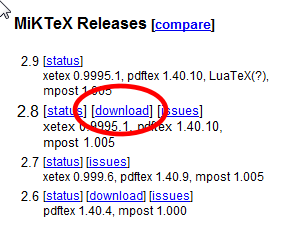
\includegraphics[scale=0.5]{miktex.png}
\end{center}

你會發現有兩個版本, 一個是 ``Basic'' MikTeX installer, 這只會裝基本套件, 我們要完整安裝, 要先選 ``Net Installer''。

\begin{center}
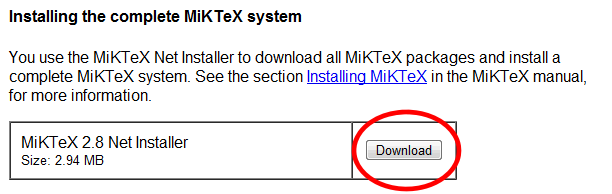
\includegraphics[scale=0.5]{miktexInstaller.png}
\end{center}

\begin{center}
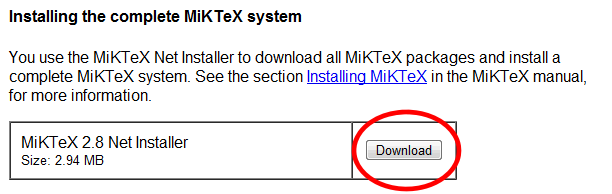
\includegraphics[scale=0.5]{miktexInstaller.png}
\end{center}

我們按下 ``Download'' 鍵之後, 會出現 MikTeX 的安裝程式。

\begin{center}
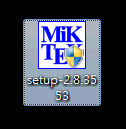
\includegraphics[scale=0.5]{miktexsetup.png}
\end{center}

開啟後, 請接受使用條款, 然後會讓你選擇要下載或安裝。我們建議先下載完整 MikTeX 再安裝, 所以請選擇 ``Download MikTeX''。

\begin{center}
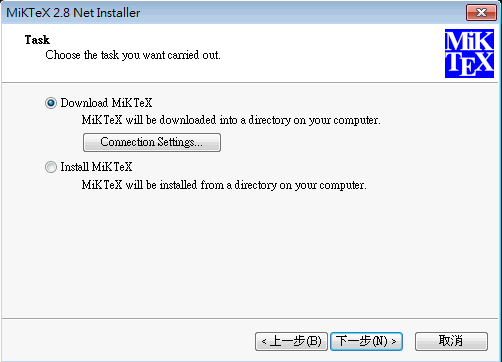
\includegraphics[scale=0.5]{DownloadMikTeX.png}
\end{center}

記得要選 ``Complete MiKTeX'', 完整下載。

\begin{center}
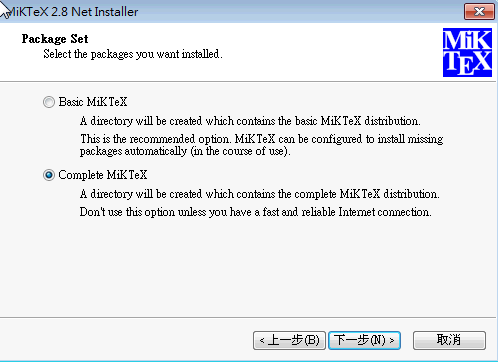
\includegraphics[scale=0.5]{Complete.png}
\end{center}

接著要選下載點, 一般就從台灣 (或所在位置) 的找一個接近的即可。

\begin{center}
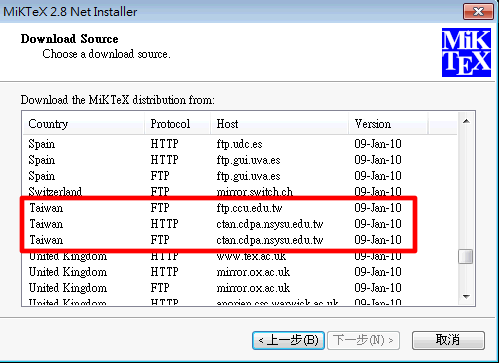
\includegraphics[scale=0.5]{source.png}
\end{center}

下載完之後, 我們{\hei{再一執行 MikTeX 的安裝程式}}, 這時候要選安裝, 並選擇完整安裝。然後程式會指向剛剛下載的地方 (當然應該和我們範例不一様), 然後一路選「下一步」就可以了。

\begin{center}
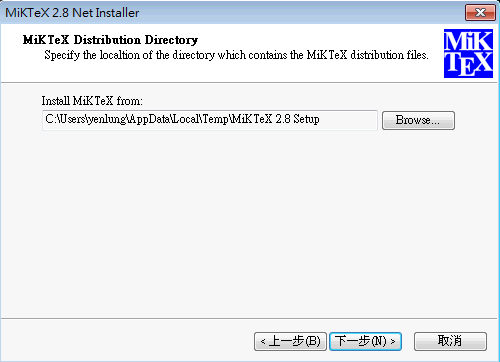
\includegraphics[scale=0.5]{miktex_install.png}
\end{center}

要下載完整的 MikTeX 要相當的時間, 如果許多人都要安裝, 可以先將完整版下載。然後以後將下載好的檔案全部拷貝給別人, 執行裡面的 \cmd{setup} 安裝程式即可。

%
\section{安裝 JabRef}
JabRef 是用來管理文獻的, 安裝也是去官網下載安裝即可。

\url{http://www.xm1math.net/texmaker/}

\begin{center}
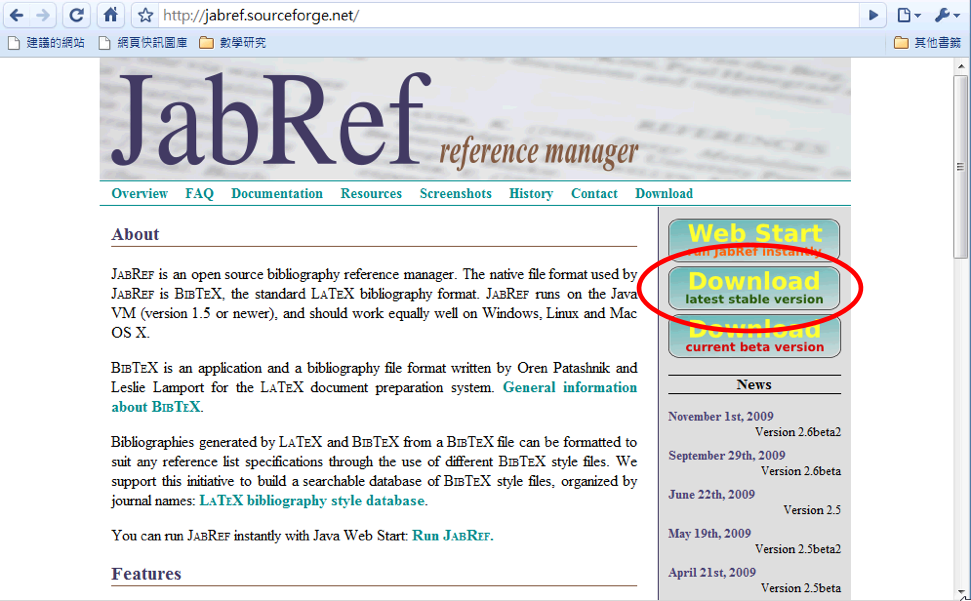
\includegraphics[scale=0.4]{windows_jabref.png}
\end{center}

唯一要注意的是, 因為 JabRef 是 Java 程式, 如果你的電腦沒有 Java 環境, 執行時會提醒你要去下載安裝 Java。

\begin{center}
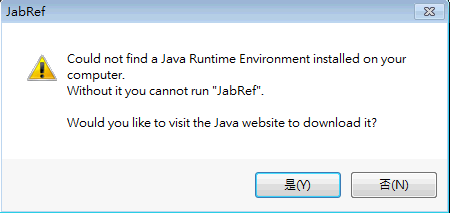
\includegraphics[scale=0.5]{windows_java.png}
\end{center}

\begin{center}
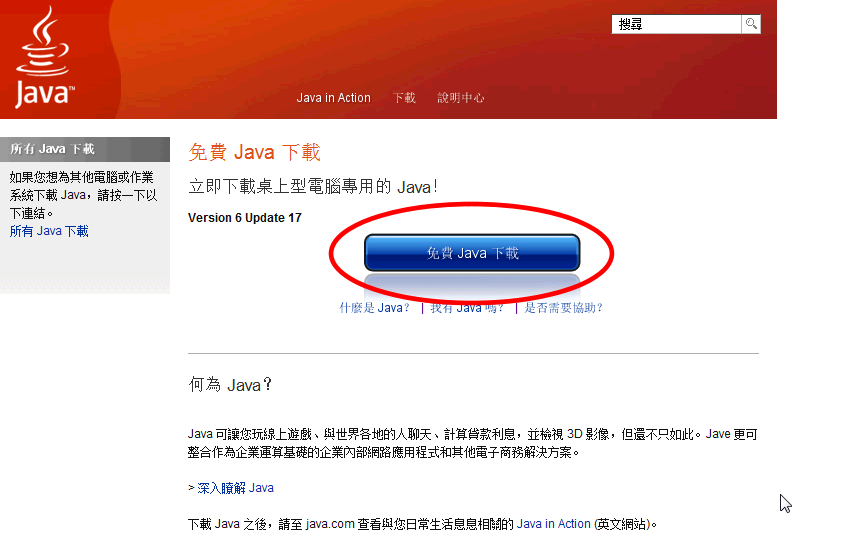
\includegraphics[scale=0.4]{windows_javadownload.png}
\end{center}

%%%
\chapter{Mac OS X 上安裝 \LaTeX{} 系統}
在 Mac OS X 上, 完整的 \LaTeX{} 系統只需要安裝:

\begin{itemize}
\item MacTeX
\item cw\TeX{} for CJK-\LaTeX 字型
\end{itemize}

第一個步驟其實就會裝好

\begin{itemize}
\item \LaTeX{} 系統
\item TeXShop \LaTeX{} 編輯器
\item BibDesk 文獻管理程式
\end{itemize}

還附送一些實用小程式。

%
\section{MacTeX 的安裝}

我們先到 CTAN 在中山大學的映射站:

\url{http://ctan.cdpa.nsysu.edu.tw/systems/mac/mactex/}

下載 MacTeX, 這個檔案很大, 請找一個有高速網路連線的地方做。

下載完成後就是標準點兩下安裝, 這樣你已經有了包括編輯程式、文獻管理程式的完整英文 \LaTeX{} 環境。

%%
\chapter{Ubuntu 下安裝 \LaTeX{} 系統}
這一章我們介紹在 Ubuntu 下安裝 \LaTeX{} 系統, 事實上所有 Linux 或其他 Unix-like 系統的安裝方式應該大同小異。你只需要用套件管理程式安裝下面三個套件, 再裝上中文字型應該就可以了:

\begin{itemize}
\item cjk-latex
\item texmaker
\item jabref
\end{itemize}

\section{\LaTeX{} 系統的安裝}
在 Ubuntu 可以用 Synaptic 來安裝新的套件。進入 Synaptic 請在系統選單下選擇「{\hei{系統$>$管理$>$Synaptic 套件管理程式}}」準備安裝套件。

\begin{center}
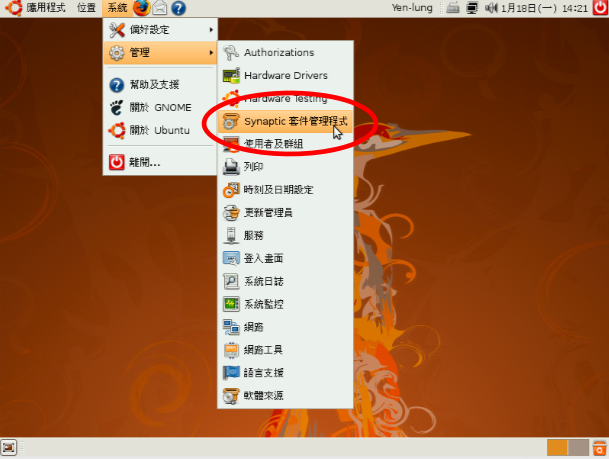
\includegraphics[scale=0.5]{ubuntu_synaptic.png}
\end{center}

我們要安裝 \cmd{ckj-latex} 套件, 事實上安裝時 Ubuntu 會把完整的 \LaTeX{} 系統都安裝好。如果在眾多套件找不到 \cmd{cjk-latex}, 請用搜尋去尋找。

\begin{center}
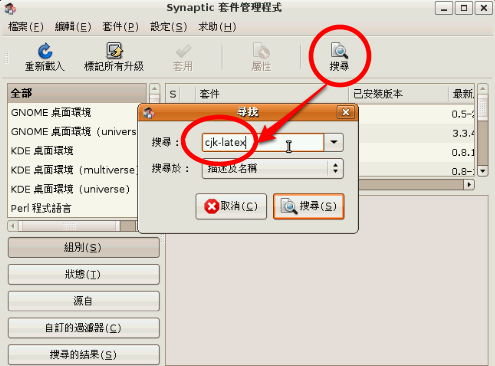
\includegraphics[scale=0.5]{ubuntu_search.png}
\end{center}

找到之後, 請在 \cmd{cjk-latex} 套件上點一下, 會出現一個選單, 請選擇「{\hei{標記為安裝}}」, 這時 Ubuntu 會準備安裝這個套件。

\begin{center}
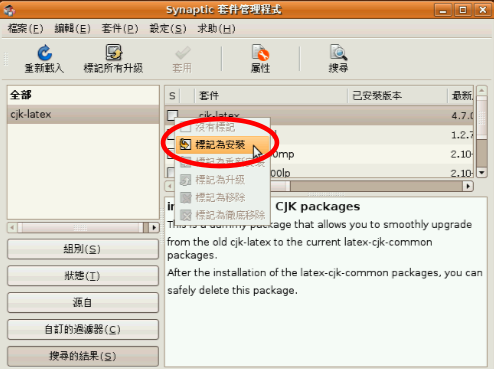
\includegraphics[scale=0.5]{ubuntu_install.png}
\end{center}

準備好了以後, 再按「{\hei{套用}}」就會安裝。

\begin{center}
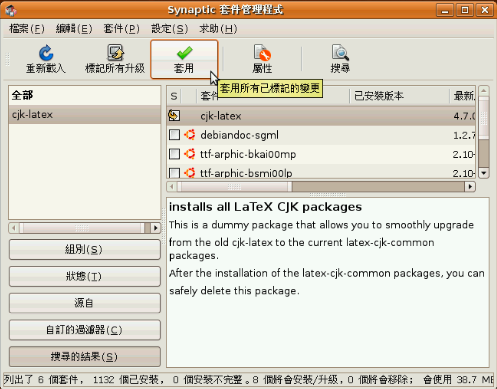
\includegraphics[scale=0.5]{ubuntu_apply.png}
\end{center}


%
\section{安裝 JabRef}

最後再安裝 \cmd{jabref}。

\begin{center}
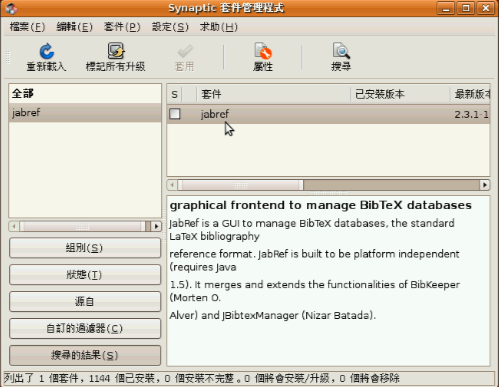
\includegraphics[scale=0.5]{ubuntu_jabref.png}
\end{center}

%
%
\chapter{\LaTeX{} 的基本介紹}
%
\section{簡單的 \LaTeX{} 文件測試}
開一個新檔, 打入下列文字。
\begin{minted}[frame=single]{latex}
\documentclass{article}
\begin{document}

Math is cool!

\end{document}
\end{minted}

當然, 中間的文字你愛打什麼打什麼, 只是暫時不要打中文。打好之後, 按下快速編譯的箭頭, 你應該就可以看到 PDF 檔。


%%%
\chapter{Xe\LaTeX{} 與 cw\TeX-Q 字型}

Xe\LaTeX{} 我在 Mac 的討論網站 Oikos 介紹過

\url{http://www.oikos.com.tw/v4/viewtopic.php?id=2939}

當時 Xe\LaTeX{} 還只有 Mac 版本, 但現在各主流平台版都有了。當時其實 Xe\LaTeX{} 還不是非常成熟, 有些文章說的現在其實不要設, 不過也許有一些朋友就照我胡說八道的方式去做了, 於是常常在網路上還是看到做了類似不必要的設定。Xe\LaTeX{} 方便的地方是, 我們不用像一般 \LaTeX{} (或 CJK-\LaTeX) 那樣, 要為 \LaTeX{} 安裝特別的字型, 直接使用系統中如 TrueType 字型等就可以! 非常方便。

但這樣子大家電腦用的字型不一樣, 文檔就難以互通。因此我們這裡推薦一個由吳聰敏、吳聰慧製作的 cw\TeX{} 字型, 經李果正整理, 再由廖鎮磐修正使字型達更佳水準的 ``cw\TeX-Q Fonts''。如果你只想直接用你系統裡的字型, 可以直接跳到~\ref{xelatex}, 否則我們就先來裝 cw\TeX-Q Fonts。

%
\section{安裝 cw\TeX-Q 字型}
首先我們先到 cw\TeX-Q 字型的網頁下載:

\url{http://code.google.com/p/cwtex-q-fonts/}

我們的目的只是要 TrueType 字型, 所以可以依指示到指定的 Google Drive 直接下載你要的版本。本文完成是最新版是 $0.3$ 版。一次可以下載所有的字型檔, 這裡要注意的是雖然有十個檔, 但其實只有五種字型。基本上是兩套不同授權方式的字型, 我們這裡都是選前面版本用的 "GNU GENERAL PUBLIC LICENSE" 那套, 你可以由字型檔名看出是哪一種授權, 詳見 cw\TeX-Q 字型官網。

五套字型的英文名稱我們等一下會用到, 所以請留意一下:

\begin{description}
\item [楷書] cwTeX Q Kai Medium
\item [黑體] cwTeX Q Hei Bold
\item [明體] cwTeX Q Ming Medium
\item [圓體] cwTeX Q Yuan Medium
\item [仿宋體] cwTeX Q Fangsong Medium
\end{description}


%
\section{Xe\LaTeX{} 中文的基本用法}\label{xelatex}
Xe\LaTeX{} 是由 Jonathan Kew 開發的, 中國南開大學孫文昌教授為 Xe\LaTeX{} 寫了對中文使用者很方便的 xeCJK 套件, 省了很多設定上的麻煩。所以我們主要介紹 xeCJK 的用法。在編譯時還是要用 Xe\LaTeX{} 編譯。

我們首先要選擇系統裡的一個字型, 找到它的名稱, 接著就照以下範例打, 就可以完全不用裝字型 (或簡單安裝如 cwTeX-Q 字型), 馬上使用中文 \LaTeX! 現在假設我們想用 cw\TeX-Q 的明體字 (\cmd{cwTeX Q Ming Medium}), 我們可以這樣做:

\begin{minted}[frame=single]{latex}
\documentclass{article}

\usepackage{xeCJK}
\setCJKmainfont{cwTeX Q Ming Medium}

\begin{document}

文章內容如一般 LaTeX, 還可打中文!

\end{document}
\end{minted}
%

所以基本上就是一般的 \LaTeX, 只有先引用套件

\begin{minted}[frame=single]{latex}
\usepackage{xeCJK}
\end{minted}

然後再設定我們要用的字型

\begin{minted}[frame=single]{latex}
\setCJKmainfont{cwTeX Q Ming Medium}
\end{minted}

就可以了!

唯一要小心是在編譯時, 我們要選用 Xe\LaTeX{} 編譯。比方說, 我們的 \LaTeX{} 檔叫 \cmd{foo.tex}, 那我們就可以這樣編譯:

\begin{minted}[frame=single]{latex}
xelatex foo.tex
\end{minted}

所以幾乎和以前是一模一樣的! 更何況像 TeXworks, TeXShop 等等 \LaTeX{} 專用文字編輯器, 都可以直接選擇用 Xe\LaTeX{} 編譯。

%
\chapter{JabRef 的基本設定}
使用 JabRef, 可以讓你的文獻管理更加容易。我們這裡介紹怎麼樣設定 JabRef。請選擇 \cmd{Options$>$Perferences} 進行偏好設定。

\begin{center}
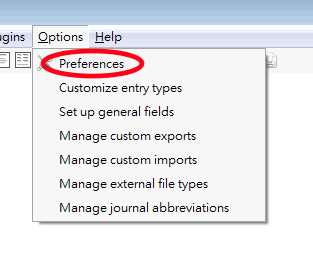
\includegraphics[scale=0.5]{jabref_pref.png}
\end{center}

\section{編碼設定}

首先, 最重要的 (尤其要用到中文), 我們要把編碼設成 UTF-8。

\begin{center}
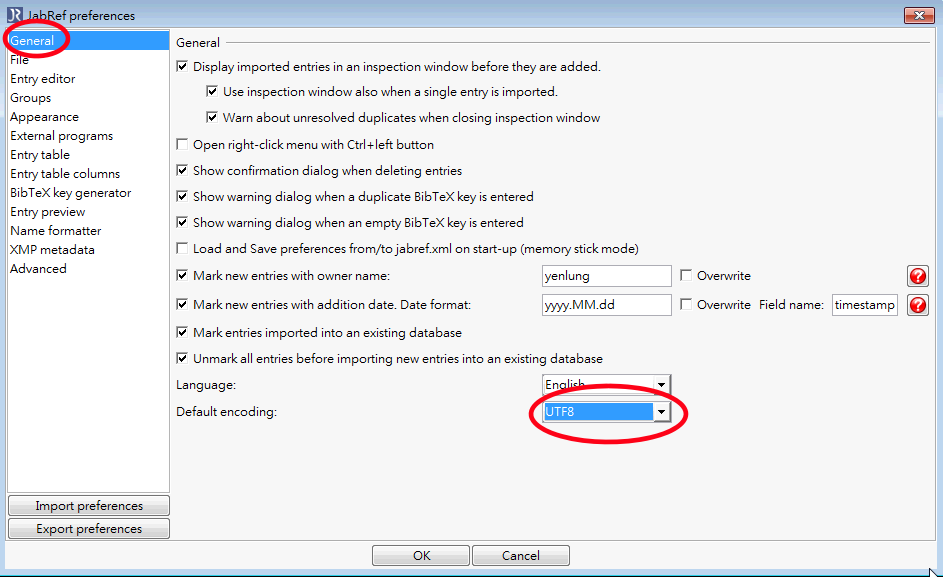
\includegraphics[scale=0.4]{jabref_encoding.png}
\end{center}

\section{引用關鍵字的設定}

我們可以設好引用關鍵字, 讓 JabRef 在你打入一篇文章後自動生成。比如說, 我們要用 \cmd{[authshort]} 達成我們要的特別引用方式:

\begin{itemize}
\item 只有一個作者時, 就用那位作者的姓當關鍵字。
\item 有二到三位作者時, 就用每一位作者姓氐的第一個字母。
\item 比三位還多時, 就列出前三位姓氐的第一個字母, 並顯示一個加號。
\end{itemize}

我們希望全部小寫, 所以用 \cmd{[authshort:lower]}。最後, 年份可以用 \cmd{[shortyear]} 顯示西元最後兩位數字。因此, 我們要在 \cmd{BibTeX key generator} 下的 \cmd{Default pattern} 輸入:

\begin{Verbatim}[frame=single]
[authshort:lower][shortyear]
\end{Verbatim}

\begin{center}
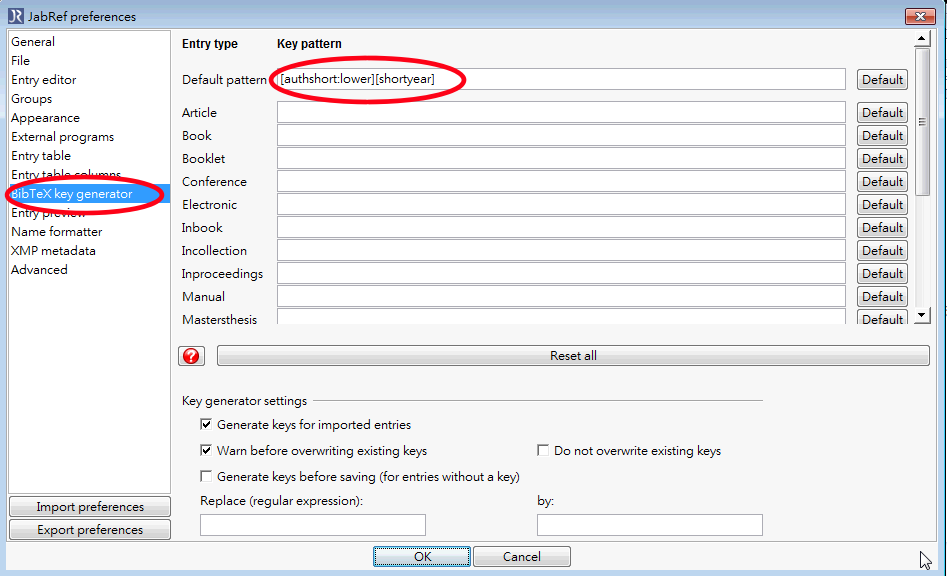
\includegraphics[scale=0.4]{jabref_bibkey.png}
\end{center}

\section{產生引用關鍵字}

一般的引入的文章, 會依我們的規則, 自動產生索引關鍵字。要是沒有自動產生, 可以選好需要產生引用關鍵字的文章, 然後按一下「魔法棒」就可以了。

\begin{center}
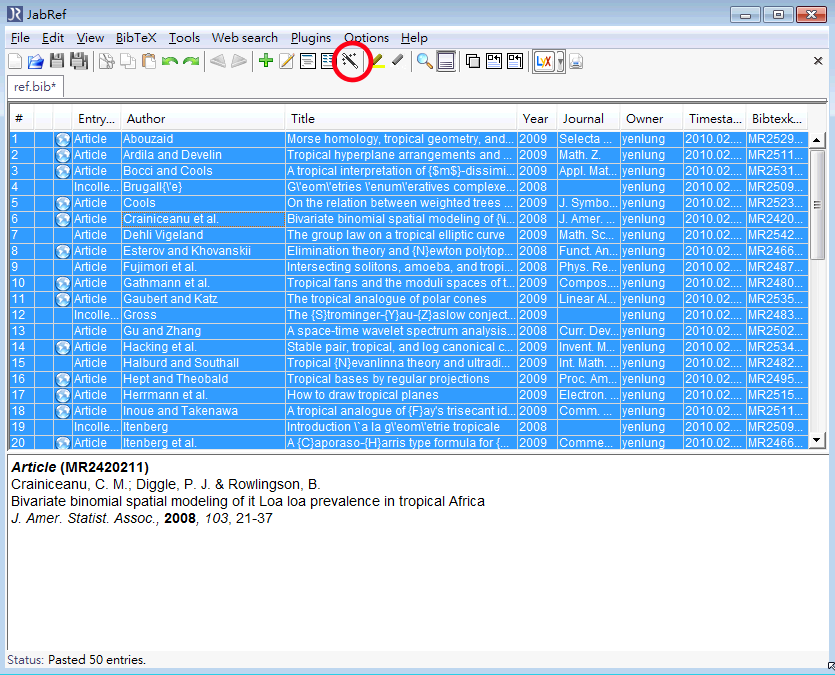
\includegraphics[scale=0.4]{jabref_auto.png}
\end{center}


\end{document}